\documentclass{standalone}
\usepackage{tikz}
\usetikzlibrary{patterns, positioning}
\usepackage[sfdefault]{ClearSans} %% option 'sfdefault' activates Clear Sans as the default text font
\usepackage[T1]{fontenc}

\begin{document}
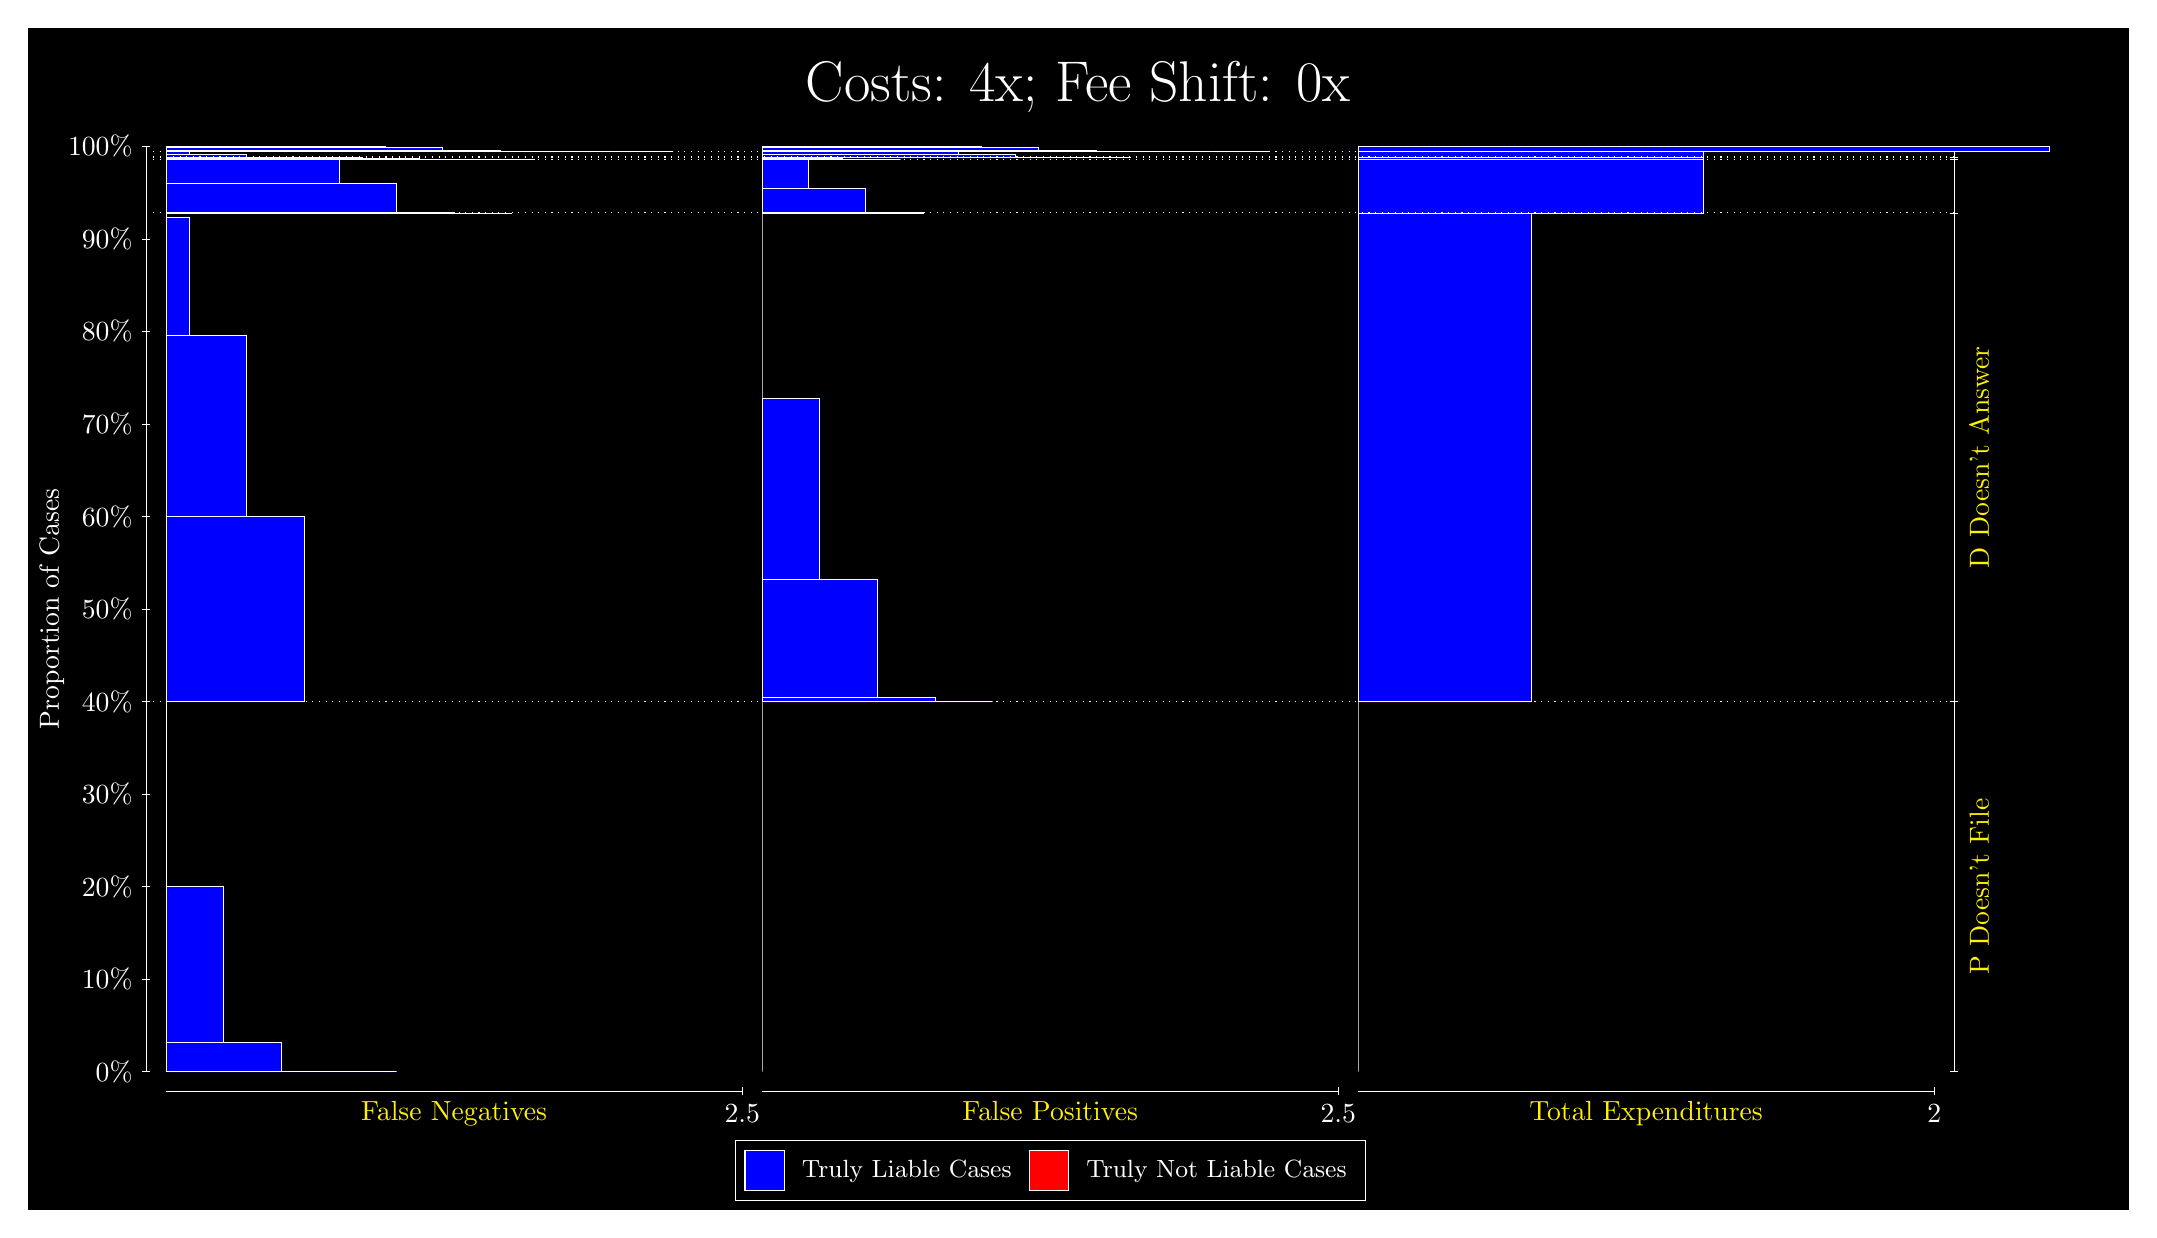
\begin{tikzpicture}
\draw[fill=black] (0,0) rectangle (26.667,15);
\draw[text=white] (0,13.5) rectangle (26.667,15) node[midway] {\huge Costs: 4x; Fee Shift: 0x};
\draw[white, very thin] (1.5,1.75) -- (1.5,13.5);
\node[rotate=90, text=white, anchor=center] at (0.3, 7.625) {Proportion of Cases};
\draw[white, very thin] (1.45,1.75) -- (1.55,1.75);
\node[text=white, anchor=east] at (1.45, 1.75) {0\%};
\draw[white, very thin] (1.45,2.925) -- (1.55,2.925);
\node[text=white, anchor=east] at (1.45, 2.925) {10\%};
\draw[white, very thin] (1.45,4.1) -- (1.55,4.1);
\node[text=white, anchor=east] at (1.45, 4.1) {20\%};
\draw[white, very thin] (1.45,5.275) -- (1.55,5.275);
\node[text=white, anchor=east] at (1.45, 5.275) {30\%};
\draw[white, very thin] (1.45,6.45) -- (1.55,6.45);
\node[text=white, anchor=east] at (1.45, 6.45) {40\%};
\draw[white, very thin] (1.45,7.625) -- (1.55,7.625);
\node[text=white, anchor=east] at (1.45, 7.625) {50\%};
\draw[white, very thin] (1.45,8.8) -- (1.55,8.8);
\node[text=white, anchor=east] at (1.45, 8.8) {60\%};
\draw[white, very thin] (1.45,9.975) -- (1.55,9.975);
\node[text=white, anchor=east] at (1.45, 9.975) {70\%};
\draw[white, very thin] (1.45,11.15) -- (1.55,11.15);
\node[text=white, anchor=east] at (1.45, 11.15) {80\%};
\draw[white, very thin] (1.45,12.325) -- (1.55,12.325);
\node[text=white, anchor=east] at (1.45, 12.325) {90\%};
\draw[white, very thin] (1.45,13.5) -- (1.55,13.5);
\node[text=white, anchor=east] at (1.45, 13.5) {100\%};

\draw[white, very thin] (24.457,1.75) -- (24.457,13.5);
\draw[white, very thin] (24.407,1.75) -- (24.507,1.75);
\node[anchor=west] at (24.407, 1.75) {};
\draw[white, very thin] (24.407,6.4489) -- (24.507,6.4489);
\node[anchor=west] at (24.407, 6.4489) {};
\draw[white, very thin] (24.407,12.656) -- (24.507,12.656);
\node[anchor=west] at (24.407, 12.656) {};
\draw[white, very thin] (24.407,13.337) -- (24.507,13.337);
\node[anchor=west] at (24.407, 13.337) {};
\draw[white, very thin] (24.407,13.365) -- (24.507,13.365);
\node[anchor=west] at (24.407, 13.365) {};
\draw[white, very thin] (24.407,13.436) -- (24.507,13.436);
\node[anchor=west] at (24.407, 13.436) {};
\draw[white, very thin] (24.407,13.5) -- (24.507,13.5);
\node[anchor=west] at (24.407, 13.5) {};

\draw[white, very thin, fill=blue] (1.75,1.75) rectangle (4.6775,1.75);
\draw[white, very thin, fill=blue] (1.75,1.75) rectangle (3.9457,1.7532);
\draw[white, very thin, fill=blue] (1.75,1.7532) rectangle (3.2138,2.126);
\draw[white, very thin, fill=blue] (1.75,2.126) rectangle (2.4819,4.1027);
\draw[white, very thin, fill=red] (1.75,4.1027) rectangle (1.75,4.1027);
\draw[white, very thin, fill=blue] (1.75,4.1027) rectangle (1.75,6.4489);
\draw[white, very thin, fill=blue] (1.75,6.4489) rectangle (3.5065,8.7984);
\draw[white, very thin, fill=blue] (1.75,8.7984) rectangle (2.7746,11.099);
\draw[white, very thin, fill=blue] (1.75,11.099) rectangle (2.0428,12.603);
\draw[white, very thin, fill=red] (1.75,12.603) rectangle (1.75,12.603);
\draw[white, very thin, fill=blue] (1.75,12.603) rectangle (1.75,12.656);
\draw[white, very thin, fill=blue] (1.75,12.656) rectangle (6.1413,12.656);
\draw[white, very thin, fill=blue] (1.75,12.656) rectangle (5.4094,12.663);
\draw[white, very thin, fill=blue] (1.75,12.663) rectangle (4.6775,13.029);
\draw[white, very thin, fill=blue] (1.75,13.029) rectangle (3.9457,13.333);
\draw[white, very thin, fill=blue] (1.75,13.333) rectangle (3.2138,13.337);
\draw[white, very thin, fill=red] (1.75,13.337) rectangle (1.75,13.337);
\draw[white, very thin, fill=blue] (1.75,13.337) rectangle (6.4341,13.337);
\draw[white, very thin, fill=blue] (1.75,13.337) rectangle (5.7022,13.337);
\draw[white, very thin, fill=blue] (1.75,13.337) rectangle (4.9703,13.351);
\draw[white, very thin, fill=blue] (1.75,13.351) rectangle (4.2384,13.365);
\draw[white, very thin, fill=blue] (1.75,13.365) rectangle (3.5065,13.365);
\draw[white, very thin, fill=red] (1.75,13.365) rectangle (1.75,13.365);
\draw[white, very thin, fill=blue] (1.75,13.365) rectangle (3.5065,13.366);
\draw[white, very thin, fill=blue] (1.75,13.366) rectangle (2.7746,13.402);
\draw[white, very thin, fill=blue] (1.75,13.402) rectangle (2.0428,13.435);
\draw[white, very thin, fill=red] (1.75,13.435) rectangle (1.75,13.435);
\draw[white, very thin, fill=blue] (1.75,13.435) rectangle (1.75,13.436);
\draw[white, very thin, fill=blue] (1.75,13.436) rectangle (8.1906,13.436);
\draw[white, very thin, fill=blue] (1.75,13.436) rectangle (7.4587,13.436);
\draw[white, very thin, fill=blue] (1.75,13.436) rectangle (6.7268,13.437);
\draw[white, very thin, fill=blue] (1.75,13.437) rectangle (5.9949,13.452);
\draw[white, very thin, fill=blue] (1.75,13.452) rectangle (5.2631,13.484);
\draw[white, very thin, fill=blue] (1.75,13.484) rectangle (4.5312,13.499);
\draw[white, very thin, fill=blue] (1.75,13.499) rectangle (3.7993,13.5);
\draw[white, very thin, fill=blue] (1.75,13.5) rectangle (3.0674,13.5);
\draw[white, very thin, fill=blue] (1.75,13.5) rectangle (2.3355,13.5);
\draw[white, very thin, fill=red] (1.75,13.5) rectangle (1.75,13.5);
\draw[white, very thin, fill=red] (9.3189,1.75) rectangle (9.3189,1.75);
\draw[white, very thin, fill=blue] (9.3189,1.75) rectangle (9.3189,6.4489);
\draw[white, very thin, fill=red] (9.3189,6.4489) rectangle (12.246,6.4489);
\draw[white, very thin, fill=blue] (9.3189,6.4489) rectangle (12.246,6.4489);
\draw[white, very thin, fill=blue] (9.3189,6.4489) rectangle (11.515,6.5013);
\draw[white, very thin, fill=blue] (9.3189,6.5013) rectangle (10.783,8.0061);
\draw[white, very thin, fill=blue] (9.3189,8.0061) rectangle (10.051,10.306);
\draw[white, very thin, fill=blue] (9.3189,10.306) rectangle (9.3189,12.656);
\draw[white, very thin, fill=red] (9.3189,12.656) rectangle (11.368,12.656);
\draw[white, very thin, fill=blue] (9.3189,12.656) rectangle (11.368,12.659);
\draw[white, very thin, fill=blue] (9.3189,12.659) rectangle (10.636,12.963);
\draw[white, very thin, fill=blue] (9.3189,12.963) rectangle (9.9044,13.33);
\draw[white, very thin, fill=blue] (9.3189,13.33) rectangle (9.3189,13.337);
\draw[white, very thin, fill=red] (9.3189,13.337) rectangle (11.075,13.337);
\draw[white, very thin, fill=blue] (9.3189,13.337) rectangle (11.075,13.337);
\draw[white, very thin, fill=blue] (9.3189,13.337) rectangle (10.344,13.351);
\draw[white, very thin, fill=blue] (9.3189,13.351) rectangle (9.6116,13.365);
\draw[white, very thin, fill=blue] (9.3189,13.365) rectangle (9.3189,13.365);
\draw[white, very thin, fill=red] (9.3189,13.365) rectangle (14.003,13.365);
\draw[white, very thin, fill=blue] (9.3189,13.365) rectangle (14.003,13.365);
\draw[white, very thin, fill=blue] (9.3189,13.365) rectangle (13.271,13.365);
\draw[white, very thin, fill=blue] (9.3189,13.365) rectangle (12.539,13.398);
\draw[white, very thin, fill=blue] (9.3189,13.398) rectangle (11.807,13.435);
\draw[white, very thin, fill=blue] (9.3189,13.435) rectangle (11.075,13.436);
\draw[white, very thin, fill=red] (9.3189,13.436) rectangle (15.759,13.436);
\draw[white, very thin, fill=blue] (9.3189,13.436) rectangle (15.759,13.436);
\draw[white, very thin, fill=blue] (9.3189,13.436) rectangle (15.028,13.436);
\draw[white, very thin, fill=red] (9.3189,13.436) rectangle (15.028,13.436);
\draw[white, very thin, fill=blue] (9.3189,13.436) rectangle (15.028,13.436);
\draw[white, very thin, fill=blue] (9.3189,13.436) rectangle (14.296,13.437);
\draw[white, very thin, fill=red] (9.3189,13.437) rectangle (14.296,13.437);
\draw[white, very thin, fill=blue] (9.3189,13.437) rectangle (14.296,13.437);
\draw[white, very thin, fill=blue] (9.3189,13.437) rectangle (13.564,13.438);
\draw[white, very thin, fill=red] (9.3189,13.438) rectangle (13.564,13.438);
\draw[white, very thin, fill=blue] (9.3189,13.438) rectangle (13.564,13.452);
\draw[white, very thin, fill=blue] (9.3189,13.452) rectangle (12.832,13.452);
\draw[white, very thin, fill=red] (9.3189,13.452) rectangle (12.832,13.452);
\draw[white, very thin, fill=blue] (9.3189,13.452) rectangle (12.832,13.484);
\draw[white, very thin, fill=blue] (9.3189,13.484) rectangle (12.1,13.499);
\draw[white, very thin, fill=blue] (9.3189,13.499) rectangle (11.368,13.5);
\draw[white, very thin, fill=blue] (9.3189,13.5) rectangle (10.636,13.5);
\draw[white, very thin, fill=blue] (9.3189,13.5) rectangle (9.9044,13.5);
\draw[white, very thin, fill=red] (16.888,1.75) rectangle (16.888,1.75);
\draw[white, very thin, fill=blue] (16.888,1.75) rectangle (16.888,6.4489);
\draw[white, very thin, fill=red] (16.888,6.4489) rectangle (19.083,6.4489);
\draw[white, very thin, fill=blue] (16.888,6.4489) rectangle (19.083,12.656);
\draw[white, very thin, fill=red] (16.888,12.656) rectangle (21.279,12.656);
\draw[white, very thin, fill=blue] (16.888,12.656) rectangle (21.279,13.337);
\draw[white, very thin, fill=red] (16.888,13.337) rectangle (21.279,13.337);
\draw[white, very thin, fill=blue] (16.888,13.337) rectangle (21.279,13.365);
\draw[white, very thin, fill=red] (16.888,13.365) rectangle (21.279,13.365);
\draw[white, very thin, fill=blue] (16.888,13.365) rectangle (21.279,13.436);
\draw[white, very thin, fill=red] (16.888,13.436) rectangle (25.67,13.436);
\draw[white, very thin, fill=blue] (16.888,13.436) rectangle (25.67,13.437);
\draw[white, very thin, fill=red] (16.888,13.437) rectangle (25.67,13.437);
\draw[white, very thin, fill=blue] (16.888,13.437) rectangle (25.67,13.5);
\draw[white, dotted] (1.5,6.4489) -- (24.457,6.4489);
\draw[white, dotted] (1.5,12.656) -- (24.457,12.656);
\draw[white, dotted] (1.5,13.337) -- (24.457,13.337);
\draw[white, dotted] (1.5,13.365) -- (24.457,13.365);
\draw[white, dotted] (1.5,13.436) -- (24.457,13.436);
\draw[white, very thin] (1.75,1.5) -- (9.0689,1.5);
\node[text=yellow, anchor=north] at (5.4094, 1.5) {False Negatives};
\draw[white, very thin] (9.0689,1.45) -- (9.0689,1.55);
\node[text=white, anchor=north] at (9.0689, 1.45) {2.5};

\draw[white, very thin] (9.3189,1.5) -- (16.638,1.5);
\node[text=yellow, anchor=north] at (12.978, 1.5) {False Positives};
\draw[white, very thin] (16.638,1.45) -- (16.638,1.55);
\node[text=white, anchor=north] at (16.638, 1.45) {2.5};

\draw[white, very thin] (16.888,1.5) -- (24.207,1.5);
\node[text=yellow, anchor=north] at (20.547, 1.5) {Total Expenditures};
\draw[white, very thin] (24.207,1.45) -- (24.207,1.55);
\node[text=white, anchor=north] at (24.207, 1.45) {2};

\node[text=yellow, centered, rotate=90] at (24.777, 4.0995) {P Doesn't File};
\node[text=yellow, centered, rotate=90] at (24.777, 9.5523) {D Doesn't Answer};





\draw (12.978300999999998,1.5) node[draw=none] (baseCoordinate) {};
\begin{scope}[align=center]
        \matrix[scale=0.5, draw=white, below=0.5cm of baseCoordinate, nodes={draw}, column sep=0.1cm]{
            \node[rectangle, draw, minimum width=0.5cm, minimum height=0.5cm, fill=blue] {}; &
            \node[draw=none, font=\small, text=white] (B) {Truly Liable Cases}; &
            \node[rectangle, draw, minimum width=0.5cm, minimum height=0.5cm, fill=red] {}; &
            \node[draw=none, font=\small, text=white] (B) {Truly Not Liable Cases}; \\
            };
\end{scope}

\end{tikzpicture}
\end{document}